\documentclass[11pt]{article}
\title{CSE 576 Project 3: Generative Discriminative Image Classifier.}
\author{Brendan Miller}
\usepackage{multirow,amsmath}
\usepackage{graphicx}
\usepackage{fancyvrb}
\usepackage{color}
\usepackage{amsfonts}
%\usepackage{hyperref}
\usepackage{longtable}
\begin{document}

\maketitle
\section{Introduction}

For this project I built a classifier that recognizes images that
contain certain classes of objects. To do this I use the
generative/discriminative framework discussed in Yi Li\cite{gendesc}.

Whereas Li's paper used features extracted from clustered regions such
as color and texture, this project also uses descriptors extracted
from keypoints. Specifically, the keypoints and descriptors
generated by SIFT.

\section{Related work}

This project is primarily based on \emph{A Generative/Discriminative
  Learning Algorithm for Image Classification} by Yi
Li\cite{gendesc}. Li's generative/discriminative classifier framework
works in two stages.

First, features are extracted from a training set of positive
examples. From this set of features, the expectation maximization
algorithm is used to create a gaussian mixture model of the
distribution of the features.

For an object $o$ and a feature type $a$ the probability of a
particular feature vector $X^a$ appearing can be calculated from the
gaussian mixture model as
\begin{equation*}
  P(X^a|o) = \sum_{m=1}^{M^a} w^a_m N(X^a; \mu^a_m, \Sigma^a_m)
\end{equation*}
where $M^a$ is the number of clusters in the mixture model for feature
$a$. For the $m$th gaussian of feature $a$ $w^a_m$ is the weight,
$\mu^a_m$ is the mean, and $\Sigma^a_m$ is the covariance matrix.

In the discriminative step, both positive and negative examples are
used to train a classifier, in this case a pretty standard 3 layer
neural network.

For the $i$th image the joint probabilities of the $r$th feature
in the image and the $m$th component gaussian of feature type $a$ is
calculated like so:
\begin{equation*}
  P(X^a_{i,r},m^a) = w^a_m N(X^a_{i,r}, \mu^a_m, \Sigma^a_m)
\end{equation*}
to determine how well an image $I_i$ matched a component gaussian
$m_a$, I just use the maximum for all features in the image. My
reasoning is that having some background features that do not match,
should reduce the score of the overall match:
\begin{equation*}
P(I_i, m^a) = max(\{P(X^a_{i,r}, m^a)|r \in \mbox{features of type $a$
  in the $i$th image\}})
\end{equation*}

For each image $I_i$ all of these maximum joint probability values
$P(I_i, m^a)$ for all components $m^a$ and all features $a$ are
aggregated into a vector. This vector is used to train a 3 layer
neural network. The neural network is trained to return 1 for vectors
from positive example images, and 0 for negative examples.

In practice, given a vector of maximum joint probabilities, the neural
network will return a value roughly between 0 and 1 that corresponds
to the confidence that object $o$ is present. For this reason, a
threshold over the output of the neural network can be varied to trade
off the likely number of false positives and false negatives
returned. In my implementation I use a threshold of 0.5.

\section{Your method}

My implementation keeps the underlying framework of Li's paper, but in
additional to using regional features mine also uses descriptors from
keypoints.

In my implementation for each image I extracted SIFT\cite{sift}
descriptors using the OpenCV library and fed these into the generative
discriminative framework discussed in the last section.

I found that using a fairly large number of component gaussians in the
SIFT mixture model helped greatly with classification accuracy. I
believe this is because a given object class can have many distinctive
parts, and a component gaussian is needed to represent the
distribution of features in each part.

For instance, in a mixture model representing the distribution of SIFT
features extracted from motorcycle images, you would want one
component gaussian to represent the descriptors extracted from
headlamps, another to represent wheels, another for tailpipes, and so
on.

Using only SIFT features and a gaussian mixture model with 50
components, I could achieve classification accuracy around 75\% to
80\%.

The number of gaussian components can continue to be increased to
increase accuracy. I capped it at 50 for most of my testing mainly
because the computational overhead in the training phase became
significant with higher numbers of gaussians.

In addition to SIFT descriptors, I also ran kmeans on each image to
extract color clusters in CIE L*a*b* color space, the mean color each
of which I fed into the generative/discriminative framework.

Color is mainly useful for classifying objects that have a distinctive
color, such as faces which contain the human skin color. They were
less useful for classifying planes, and motorcycles, all of which can
be painted a variety of colors. Cars were well classified by color;
however as I discuss in the experimental results I think this has more
to do with the uniformity of the car data set than anything else.

\section{Experiments and results}

I used motor bikes, faces, airplanes, and cars from the caltech image
sets linked from the original project description. 

Links to datasets used for testing:
\begin{verbatim}
http://www.vision.caltech.edu/Image_Datasets/cars_brad/cars_brad.tar
http://www.vision.caltech.edu/Image_Datasets/motorbikes_side/motorbikes_side.tar
http://www.vision.caltech.edu/Image_Datasets/airplanes_side/airplanes_side.tar
http://www.vision.caltech.edu/Image_Datasets/faces/faces.tar
\end{verbatim}

I use a training set of 400 images and a test set of 200 images
randomly selected from a larger collection. Each set contains 50/50
positive and negative examples.

For the data collected here I used a gaussian mixture model with 10
components to represent the color distribution of each class and a
mixture model with 50 components to represent the SIFT feature
distribution.

\subsection{SIFT features only}

Using SIFT alone performance was pretty decent across a range of image
types. In general increasing the number of gaussians in the mixture
model improves SIFT at the expense of additional training time.

\begin{tabular}{| l | l | l | l |}
  \hline
  Image Type & Accuracy     & False Positives    & False Negatives \\
  Cars      & 0.735 & 0.125 & 0.14  \\
  Planes    & 0.775 & 0.09  & 0.135 \\
  Faces     & 0.78  & 0.13  & 0.09  \\
  Bikes     & 0.755 & 0.11  & 0.135 \\
  \hline
\end{tabular}

\subsection{CIE L*a*b* color features only}

Not surprisingly faces do a little bit better than planes and
motorcycles when only using color for image classification, as faces
have a fairly distinctive color tone that has been shown to be well
modeled by a gaussian distribution. By comparison planes and
motorcycles can be painted a variety of arbitrary colors.

What is most surprising is that cars are classified so well by color
alone. My suspicion is that this is because the training images shows
cars as they are driving surrounded by pavement, and that the color
of the pavement is really what the classifier is finding. This belief
is given further evidence because many false positives were non-car
images that had pavement in them.

For this reason I consider the motorcycle data a lot better
representation of the power of this model, as it has motorcycles in a
variety of scenes, including scenes where the background has been
cropped out.

\begin{tabular}{| l | l | l | l |}
  \hline
  Image Type & Accuracy     & False Positives    & False Negatives \\
  Cars      & 0.905 & 0.085 & 0.01  \\
  Planes    & 0.77  & 0.075 & 0.155 \\
  Faces     & 0.795 & 0.095 & 0.11  \\
  Bikes     & 0.725 & 0.19  & 0.085 \\
  \hline
\end{tabular}

\subsection{Combined SIFT and CIE L*a*b* color features}

This set of results really shows the strength of the discriminative
generative model. Every result is a bit better than the results from
the individual features. Face classification in particular really
benefits from a combination of both color and keypoint descriptor
data.

\begin{tabular}{| l | l | l | l |}
  \hline
  Image Type & Accuracy     & False Positives    & False Negatives \\
  Cars      & 0.94  & 0.035 & 0.025 \\
  Planes    & 0.78  & 0.11  & 0.11  \\
  Faces     & 0.9   & 0.055 & 0.045 \\
  Bikes     & 0.805 & 0.08  & 0.115 \\
  \hline
\end{tabular}

This is an example of a correctly classified plane.

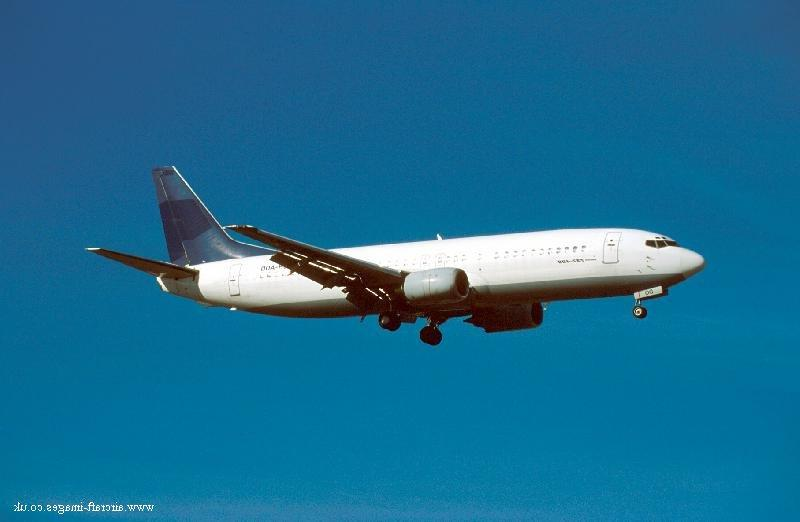
\includegraphics[width=100mm]{images/plane_true_positive.png}

False positives:
It's a little tricky to interpret why this example was classified as a
plane, but my guess is that the white color of the car, which is more
common on commercial aircraft then in automobiles, partially had to do
with it.

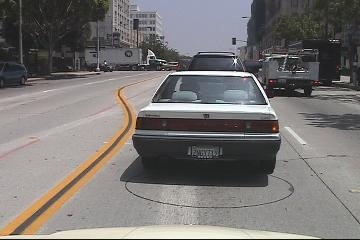
\includegraphics[width=100mm]{images/plane_false_positive.png}

False negatives:
Here's an example of a false negative during face classification. This
image lacks the distinctive color of skin, and is also hand drawn so
keypoint descriptors may not be quite the same as with real faces.

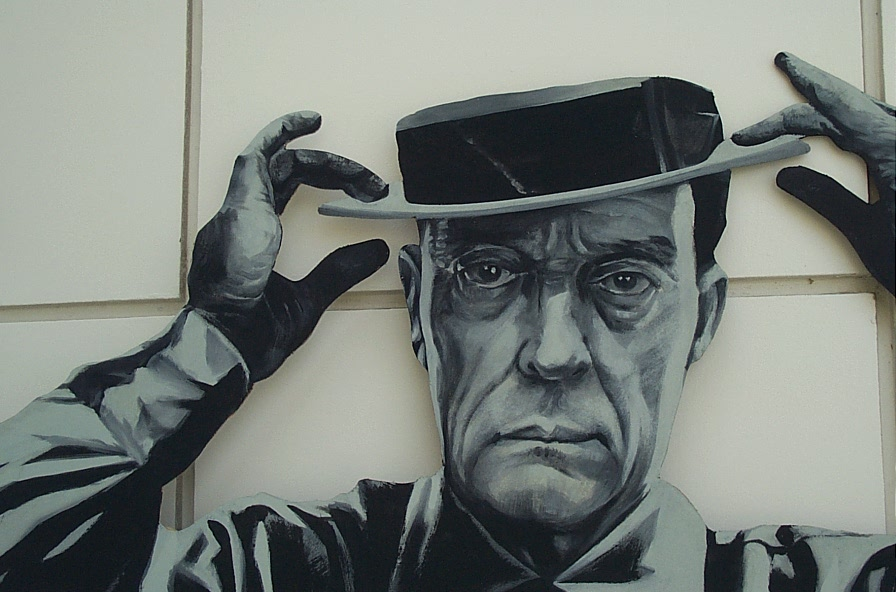
\includegraphics[width=100mm]{images/face_false_negative.png}


\section{Future work}

One idea to extend this project would be to try to work backwards from an
image classified as having an object, to try to find which features
were responsible for the positive classification.

If some book-keeping were done to keep track of the locations and size
of the original features, a bounding box around the region likely
containing the object could be found.

One obstacle to this approach is that the fairly complex structure of
a 3 layer neural network is a little tricky to interpret when trying
to determine which input data is responsible for the result. For
that reason experiments with either a 2 layer network, or some other
simpler classifier could be done.

My intuition is that a 3 layer network may be more powerful than
necessary for the generative discriminative framework, though further
testing is necessary to confirm this.

\section{Summary and conclusion}

I've used this project to combine both regional and keypoint
descriptor data to form a bag of words classifier.

My experimental results confirm that very disparate kinds of features
can be effectively combined by the generative discriminative framework
to improve performance. Indeed, probably the most effective use of the
framework is to combine feature types that have as little overlap as
possible in what they describe.

\section{Compiling and Running The Executable}

See the README file included with the source for instructions on
compiling and running the object recognition program.

\begin{thebibliography}{9}

\bibitem{gendesc}
  Y. Li, L. G. Shaprio, and J. Bilmes
  \emph{A Generative/Discriminative Learning Algorithm for Image Classification}.
  Department of Computer Science and Engineering,
  Department of Electrical Engineering,
  University of Washington

\bibitem{sift}
  David G. Lowe
  \emph{Distinctive Image Features from Scale-Invariant Keypoints}
  Computer Science Department
  University of British Columbia
  Vancouver, B.C., Canada
  January 5, 2004

\end{thebibliography}

\end{document}
